\documentclass[12pt]{report}
\usepackage[utf8]{inputenc}
\usepackage[russian]{babel}
%\usepackage[14pt]{extsizes}
\usepackage{listings}
\usepackage{amsmath}
\usepackage[justification=centering]{caption}

% Для листинга кода:
\lstset{ %
language=c,                 % выбор языка для подсветки (здесь это С)
basicstyle=\footnotesize\sffamily, % размер и начертание шрифта для подсветки кода
numbers=left,               % где поставить нумерацию строк (слева\справа)
numberstyle=\tiny,           % размер шрифта для номеров строк
stepnumber=1,                   % размер шага между двумя номерами строк
numbersep=5pt,                % как далеко отстоят номера строк от подсвечиваемого кода
showspaces=false,            % показывать или нет пробелы специальными отступами
showstringspaces=false,      % показывать или нет пробелы в строках
showtabs=false,             % показывать или нет табуляцию в строках
frame=single,              % рисовать рамку вокруг кода
tabsize=2,                 % размер табуляции по умолчанию равен 2 пробелам
captionpos=t,              % позиция заголовка вверху [t] или внизу [b] 
breaklines=true,           % автоматически переносить строки (да\нет)
breakatwhitespace=false, % переносить строки только если есть пробел
escapeinside={\#*}{*)}   % если нужно добавить комментарии в коде
}

\usepackage{hyperref}
\hypersetup{
    linktoc=all,     %set to all if you want both sections and subsections linked
    linkcolor=blue,  %choose some color if you want links to stand out
}

% Для измененных титулов глав:
\usepackage{titlesec, blindtext, color} % подключаем нужные пакеты
\definecolor{gray75}{gray}{0.75} % определяем цвет
\newcommand{\hsp}{\hspace{20pt}} % длина линии в 20pt
% titleformat определяет стиль
\titleformat{\chapter}[hang]{\Huge\bfseries}{\thechapter\hsp\textcolor{gray75}{|}\hsp}{0pt}{\Huge\bfseries}

% plot
\usepackage{pgfplots}
\usepackage{filecontents}
\usetikzlibrary{datavisualization}
\usetikzlibrary{datavisualization.formats.functions}


\begin{document}
\begin{titlepage}
	\fontsize{12pt}{12pt}\selectfont
	\noindent \begin{minipage}{0.15\textwidth}
		
\includegraphics[width=\linewidth]{inc/img/b_logo.jpg}
	\end{minipage}
	\noindent\begin{minipage}{0.9\textwidth}\centering
		\textbf{Министерство науки и высшего образования Российской Федерации}\\
		\textbf{Федеральное государственное бюджетное образовательное учреждение высшего образования}\\
		\textbf{«Московский государственный технический университет имени Н.Э.~Баумана}\\
		\textbf{(национальный исследовательский университет)»}\\
		\textbf{(МГТУ им. Н.Э.~Баумана)}
	\end{minipage}
	
	\noindent\rule{15cm}{3pt}
	\newline\newline
	\noindent ФАКУЛЬТЕТ \underline{~~~~~~~~~~~~~~~~«Информатика и системы управления»~~~~~~~~~~~~~~~~} \newline\newline
	\noindent КАФЕДРА \underline{«Программное обеспечение ЭВМ и информационные технологии»}\newline\newline\newline\newline\newline\newline\newline
	
	
	\begin{center}
		\Large\textbf{Отчет по лабораторной работе №5 по курсу "Анализ алгоритмов"}\newline
	\end{center}
	
	\noindent\textbf{Тема} \underline{Конвейер}\newline\newline\newline
	\noindent\textbf{Студент} \underline{Якуба Д. В.}\newline\newline
	\noindent\textbf{Группа} \underline{ИУ7-53Б}\newline\newline
	\noindent\textbf{Оценка (баллы)} \underline{~~~~~~~~~~~~~~~~~~~}\newline\newline
	\noindent\textbf{Преподаватели} \underline{Волкова Л.Л., Строганов Ю.В.}\newline
	
	\begin{center}
		\vfill
		Москва~---~\the\year
		~г.
	\end{center}
\end{titlepage}

\setcounter{page}{2}

\tableofcontents

\newpage
\chapter*{Введение}
\addcontentsline{toc}{chapter}{Введение}
\section*{Цель лабораторной работы}
Изучение и реализация асинхронного взаимодействия потоков.
\section*{Задачи лабораторной работы}
\begin{enumerate}
\item изучить асинхронное взаимодействие на примере конвейерной обработки данных;
\item спроектировать систему конвейерных вычислений;
\item реализовать систему конвейерных вычислений;
\item протестировать реализованную систему;
\item подготовить отчёт по проведенной работе.
\end{enumerate}

\chapter{Аналитическая часть}
В данном разделе описаны принцип и идея конвейерной обработки данных, а также алгоритм Брезенхема с действительными коэффициентами.

Работа алгоритма Брезенхема основывается на использовании понятия ошибка. Ошибкой здесь называется расстояние между действительным положением отрезка и ближайшим пикселем сетки растра, который аппроксимирует отрезок на очередном шаге.

На каждом шаге вычисляется величина ошибки и в зависимости от полученного значения выбирается пиксель, ближе расположенный к идеальному отрезку. Поскольку при реализации алгоритма на ЭВМ удобнее анализировать не само значение ошибки, а ее знак, то истинное значение ошибки смещается на -0,5.

Поскольку на первом шаге высвечивается пиксел с начальными координатами, то для него ошибка равняется 0, поэтому задаваемое предварительно значение этой ошибки:



\section{Конвейерная обработка данных}
Конвейерный принцип обработки данных подразумевает, что в каждый момент времени процессор работает над различными стадиями выполнения нескольких команд, причем на выполнение каждой стадии выделяются отдельные аппаратные ресурсы. Такая обработка оптимизирует использование ресурсов для заданного набора процессов, каждый из которых применяет эти ресурсы заранее предусмотренным способом.
Идея конвейерной обработки данных заключается в параллельном выполнении нескольких инструкций процессора. Сложные инструкции процессора представляются в виде последовательности более простых стадий. Вместо выполнения инструкций последовательно (ожидания завершения конца одной инструкции и перехода к следующей), следующая инструкция может выполняться через несколько стадий выполнения первой инструкции. Это позволяет управляющим цепям процессора получать инструкции со скоростью самой медленной стадии обработки, однако при этом намного быстрее, чем при выполнении эксклюзивной полной обработки каждой инструкции от начала до конца.

\section{Алгоритм Брезенхема с действительными коэффициентами}
Алгоритм Брезенхема — это алгоритм, определяющий, какие точки двумерного растра нужно закрасить, чтобы получить близкое приближение прямой линии между двумя заданными точками.

Работа алгоритма Брезенхема основывается на использовании понятия ошибка. Ошибкой здесь называется расстояние между действительным положением отрезка и ближайшим пикселем сетки растра, который аппроксимирует отрезок на очередном шаге.

На каждом шаге вычисляется величина ошибки и в зависимости от полученного значения выбирается пиксель, ближе расположенный к идеальному отрезку. Поскольку при реализации алгоритма на ЭВМ удобнее анализировать не само значение ошибки, а ее знак, то истинное значение ошибки смещается на -0,5.

Поскольку на первом шаге высвечивается пиксел с начальными координатами, то для него ошибка равняется 0, поэтому задаваемое предварительно значение этой ошибки:

\begin{equation}
\label{1:mistake}
	{mistake}= \frac{\symup\Delta y}{\symup\Delta x} - \frac{1}{2}
\end{equation}

Выражение \ref{1:mistake} фактически определяет ошибку для следующего шага.

В общем алгоритме Брезенхема большее по модулю из приращений принимается равным шагу растра, то есть единице, причем знак приращения совпадает со знаком разности конечной и начальной координат отрезка:

\begin{equation}
\label{1:deltaX}
	\symup\Delta x = sign(x_e - x_s), \textbf{если } |x_e-x_s|\geq|y_e-y_s|
\end{equation}

\begin{equation}
\label{1:deltaY}
	\symup\Delta y = sign(y_e - y_s), \textbf{если } |y_e-y_s|\geq|x_e-x_s|
\end{equation}

В выражениях \ref{1:deltaX}, \ref{1:deltaY} $x_e$ и $y_e$ - координаты начала отрезка, а $sign$ - кусочно постоянная функция действительного аргумента.

Значение другой координаты идеального отрезка для следующего шага определяется как \ref{1:ideal}, поскольку приращение ординаты совпадает с величиной одного катета прямоугольного треугольника, а другой катет равен шагу сетки растра, то есть единице.

\begin{equation}
\label{1:ideal}
	y_{ideal_i} = y_{ideal_{i + 1}} + \frac{\symup\Delta y}{\symup\Delta x}
\end{equation}

Ошибка на очередном вычисляется как:

\begin{equation}
\label{1:mistake:2}
	{mistake}_{i + 1} = y_{{ideal}_{i + 1}} - y_{i + 1} = y_{{ideal}_i} + \frac{\symup\Delta y}{\symup\Delta x} - y_i = mistake_i + \frac{\symup\Delta y}{\symup\Delta x}
\end{equation}

В зависимости от полученного значения ошибки выбирается пиксел с той же ординатой (при ошибке $< $0) или пиксел с ординатой, на единицу большей, чем у предыдущего пиксела (при ошибке $\geq0$).

Поскольку предварительное значение ошибки вычисляется заранее, то во втором случае останется только вычесть единицу из значения ошибки, так как в этом случае $y_{i+1}=y_{i} + 1$, что не учитывалось при расчете.

\section*{Вывод}
Были рассмотрены принцип и идея конвейерной обработки данных, а также алгоритм Брезенхема с действительными коэффициентами.

В данной работе стоит задача реализации системы конвейерной обработки данных для рассмотренного алгоритма.

\chapter{Конструкторская часть}
В данном разделе представлены схемы алгоритма Брезенхема и реализации конвейерной обработки данных для алгоритма Брезенхема.
\section{Схема алгоритма Брезенхема}
Схема алгоритма Брезенхема предоставлена на рисунках \ref{img:bresAlg}, \ref{img:bresAlgPart}.

\begin{figure}
\begin{center}
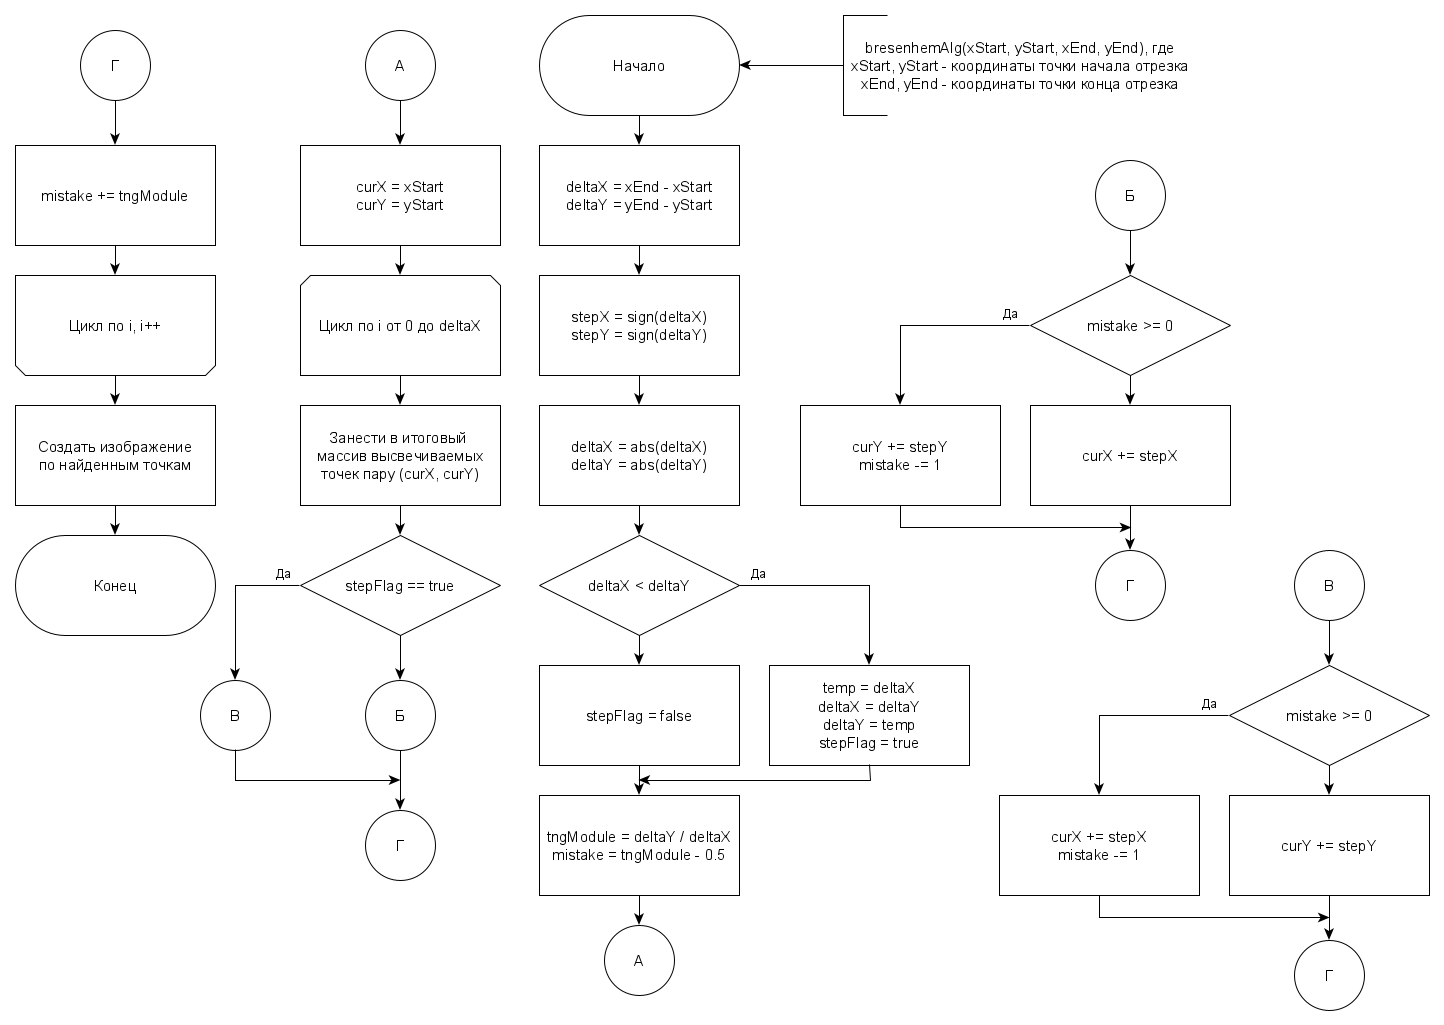
\includegraphics[scale=0.4]{inc/img/bresAlg.png}
\captionsetup{justification=centering}
	\caption{Схема алгоритма Брезенхема.}
	\label{img:bresAlg}	
\end{center}
\end{figure}

\begin{figure}
\begin{center}
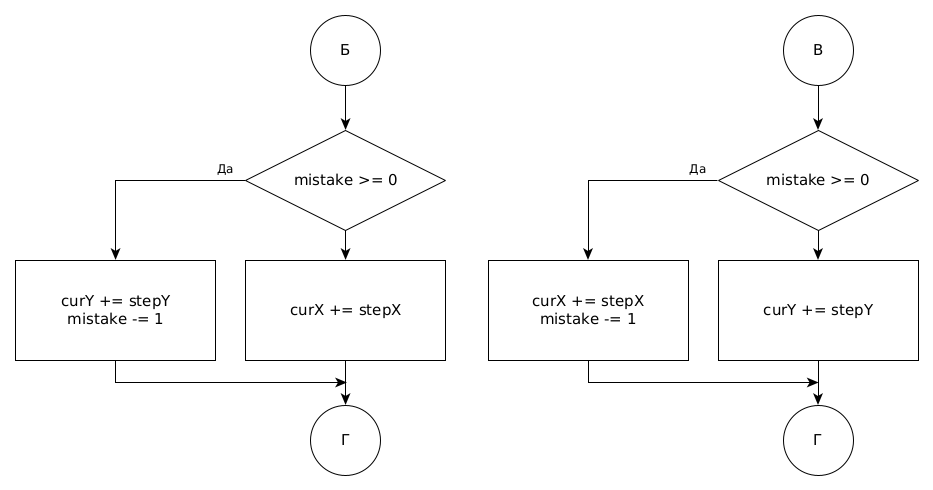
\includegraphics[scale=0.4]{inc/img/bresAlgPart.png}
\captionsetup{justification=centering}
	\caption{Схема алгоритма Брезенхема.}
	\label{img:bresAlgPart}	
\end{center}
\end{figure}

\section{Схема реализации конвейерной обработки данных для алгоритма Брезенхема}
На рисунке \ref{img:conveyor} предоставлена схема алгоритма работы функции, запускающей в требуемом количестве потоков функцию-аргумент.

\begin{figure}
\begin{center}
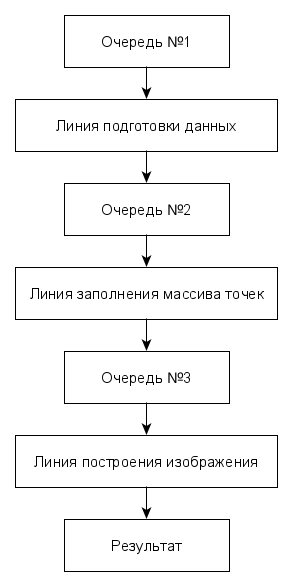
\includegraphics[scale=0.35]{inc/img/conveyor.png}
\captionsetup{justification=centering}
	\caption{Схема реализации конвейерной обработки данных для алгоритма Брезенхема.}
	\label{img:conveyor}	
\end{center}
\end{figure}

\section*{Вывод}
Были представлены схемы алгоритма Брезенхема, а также реализации конвейерной обработки данных для данного алгоритма.

\chapter{Технологическая часть}
В данном разделе приведены требования к программному обеспечению, средства реализации программного обеспечения, а также листинг кода.

\section{Требования к программному обеспечению}
\begin{itemize}
\item входные данные - количество выполняемых задач (количество растеризуемых отрезков);
\item выходные данные - записи времени прихода и ухода обрабатываемых заявок для каждого реализованного конвейера.
\end{itemize}

\section{Средства реализации программного обеспечения}
При написании программного продукта был использован язык программирования C++.

Данный выбор обусловлен следующими факторами:
\begin{itemize}
\item Данный язык программирования преподавался в рамках курса объектно-ориентированного программирования;
\item Высокая вычислительная производительность;
\item Большое количество справочной и учебной литературы в сети Интернет.
\end{itemize}

При написании программного продукта использовалась среда разработки QT Creator.

Данный выбор обусловлен следующими факторами:
\begin{itemize}
\item Основы работы с данной средой разработки преподавался в рамках курса программирования на Си;
\item QT Creator позволяет работать с расширением QtDesign.
\end{itemize}

\section{Листинг кода}
В листингах \ref{list:bresAlg} и \ref{list:director} предоставлены реализации рассматриваемых алгоритмов.
\begin{lstlisting}[caption=Разбиение алгоритма Брезенхема,
label={list:bresAlg}]
std::string now_str()
{
    const boost::posix_time::ptime now = boost::posix_time::microsec_clock::local_time();

    const boost::posix_time::time_duration td = now.time_of_day();

    const long hours = td.hours();
    const long minutes = td.minutes();
    const long seconds = td.seconds();
    const long nanoseconds =
        td.total_nanoseconds() - ((hours * 3600 + minutes * 60 + seconds) * 1000000000);

    char buf[40];
    sprintf(buf, "%02ld:%02ld:%02ld.%09ld", hours, minutes, seconds, nanoseconds);

    return buf;
}

SegmentRasterizator::SegmentRasterizator(int xStart_, int yStart_, int xEnd_, int yEnd_)
{
    xStart = xStart_;
    yStart = yStart_;
    xEnd = xEnd_;
    yEnd = yEnd_;
    if (xStart == xEnd)
        xEnd += 1;
    else if (yStart == yEnd)
        yEnd += 1;

    image = new QImage(WIDTH, HEIGHT, QImage::Format_RGB32);
    image->fill(Qt::white);
}

int sign(float num)
{
    return (num < -__FLT_EPSILON__) ? -1 : ((num > __FLT_EPSILON__) ? 1 : 0);
}

void SegmentRasterizator::prepareConstantsForRB(int index)
{
    std::printf(ANSI_BLUE_BRIGHT "From START worker: task %d BEGIN %s" ANSI_RESET "\n", index, now_str().c_str());

    deltaX = xEnd - xStart;
    deltaY = yEnd - yStart;

    stepX = sign(deltaX);
    stepY = sign(deltaY);

    deltaX = std::abs(deltaX);
    deltaY = std::abs(deltaY);

    if (deltaX < deltaY)
    {
        std::swap(deltaX, deltaY);
        stepFlag = true;
    }
    else
        stepFlag = false;

    tngModule = deltaY / deltaX;
    mistake = tngModule - 0.5;

    std::printf(ANSI_BLUE_BRIGHT "From START worker: task %d ENDED %s" ANSI_RESET "\n", index, now_str().c_str());
}

void SegmentRasterizator::rastSegment(int index)
{
    std::printf(ANSI_MAGENTA_BRIGHT "From MIDDLE worker: task %d BEGIN %s" ANSI_RESET "\n", index, now_str().c_str());

    float curX = xStart, curY = yStart;
    for (int i = 0; i <= deltaX; i++)
    {
        dotsOfSegment.push_back(std::pair<int, int>(curX, curY));
        if (stepFlag)
        {
            if (mistake >= 0)
                (curX += stepX, mistake--);
            curY += stepY;
        }
        else
        {
            if (mistake >= 0)
                (curY += stepY, mistake--);
            curX += stepX;
        }
        mistake += tngModule;
    }

    std::printf(ANSI_MAGENTA_BRIGHT "From MIDDLE worker: task %d ENDED %s" ANSI_RESET "\n", index, now_str().c_str());
}

void SegmentRasterizator::createImg(int index)
{
    std::printf(ANSI_CYAN_BRIGHT"From END worker: task %d BEGIN %s" ANSI_RESET "\n", index, now_str().c_str());

    for (auto iter = dotsOfSegment.begin(); iter < dotsOfSegment.end(); iter++)
        image->setPixel(iter->first, iter->second, Qt::black);

    std::printf(ANSI_CYAN_BRIGHT "From END worker: task %d ENDED %s" ANSI_RESET "\n", index, now_str().c_str());
}

std::vector<std::pair<int, int>> SegmentRasterizator::getDotsOfSegment()
{
    return dotsOfSegment;
}
\end{lstlisting}

\begin{lstlisting}[caption=Менеджер потоков,
label={list:director}]
Director::Director(std::queue<SegmentRasterizator> &startQueue_)
{
    startQueue = startQueue_;
}

void Director::processPrepare()
{
    int i = 0;
    for (SegmentRasterizator curSeg(startQueue.front()); startQueue.size();
         startQueue.pop(), curSeg = startQueue.front())
    {

        curSeg.prepareConstantsForRB(i++);
        middleQueue.push(curSeg);
    }
}

void Director::processRast()
{
    int i = 0;
    while (startQueue.size() || middleQueue.size())
    {
        if (middleQueue.empty())
            continue;
        SegmentRasterizator curSeg(middleQueue.front());

        curSeg.rastSegment(i++);

		endQueue.push(curSeg);
        middleQueue.pop();
    }
}

void Director::processCreate()
{
    int i = 0;
    while (startQueue.size() || middleQueue.size() || endQueue.size())
    {
        if (endQueue.empty())
            continue;
        SegmentRasterizator curSeg(endQueue.front());

        curSeg.createImg(i++);
        endQueue.pop();
        final.push_back(curSeg);
    }
}

void Director::initWork()
{
    workers[0] = std::thread(&Director::processPrepare, this);
    workers[1] = std::thread(&Director::processRast, this);
    workers[2] = std::thread(&Director::processCreate, this);

    workers[0].join();
    workers[1].join();
    workers[2].join();
}

std::vector<SegmentRasterizator> Director::getFinal() { return final; }
\end{lstlisting}

\section{Тестирование программного продукта}
В таблице~\ref{tabular:test_rec} приведены тесты для функций, реализующих алгоритм Брезенхема. Тесты пройдены успешно.

\begin{table}[h!]
	\begin{center}
	
	\caption{\label{tabular:test_rec} Тестирование функций}
		\begin{tabular}{c@{\hspace{7mm}}c@{\hspace{7mm}}c@{\hspace{7mm}}c@{\hspace{7mm}}c@{\hspace{7mm}}c@{\hspace{7mm}}}
			\hline
			Точка начала отрезка (x, y) & Точка конца отрезка (x, y) & Ожидаемый результат \\ \hline
			\vspace{4mm}
			 (1, 1)&
			 (3, 3)&
			 (1, 1), (2, 2), (3, 3)\\
			\vspace{2mm}
			\vspace{2mm}
			 (1, 1)&
			 (1, 3)&
			 (1, 1), (1, 2), (1, 3)\\
			\vspace{2mm}
			\vspace{2mm}
			 (1, 1)&
			 (2, 1)&
			 (1, 1), (2, 1)\\
			\vspace{2mm}
			\vspace{2mm}
			 (3, 3)&
			 (1, 1)&
			 (1, 1), (2, 2), (3, 3)\\
		\end{tabular}
	\end{center}
\end{table}
\section*{Вывод}
Спроектированные алгоритмы были реализованы и протестированы.

\chapter{Исследовательская часть}
\section{Технические характеристики}
Технические характеристики ЭВМ, на котором выполнялись исследования:
\begin{itemize}
\item ОС: Manjaro Linux 20.1.1 Mikah
\item Оперативная память: 16 Гб
\item Процессор: Intel Core i7-10510U
\end{itemize}

При проведении замеров времени ноутбук был подключен к сети электропитания.

\section{Пример работы программного обеспечения}
На рисунке \ref{img:example} приведен пример работы программы для 7 визуализируемых отрезков.

\begin{figure}
\begin{center}
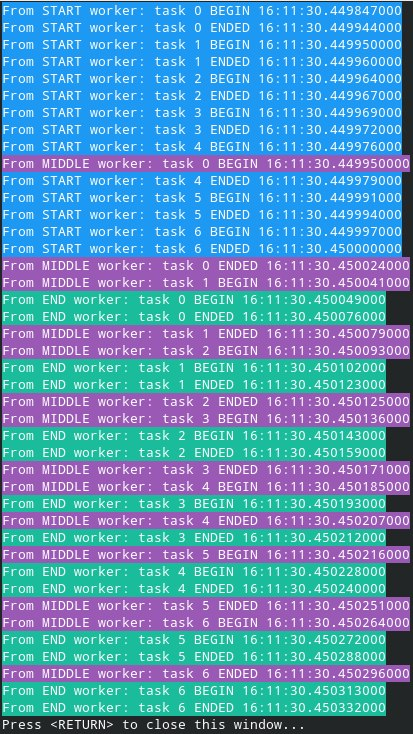
\includegraphics[scale=0.9]{inc/img/example.png}
\captionsetup{justification=centering}
	\caption{Пример работы ПО.}
	\label{img:example}	
\end{center}
\end{figure}

\newpage
\section{Время выполнения алгоритмов}
Алгоритм тестировался на данных, сгенерированных случайным образом.

В таблице \ref{time1} предоставлено время работы над каждым отрезком в предоставленном примере каждого из выделенных этапов.

Из таблицы видно, что среднее время выполнения этапа 1 составляет $\approx 17428.6$ наносекунд. Среднее время выполнения этапа 2 составляет $\approx 38285.7$ наносекунд. Среднее время выполнения этапа 3 составляет $\approx 18571.4$ наносекунд. Таким образом, этап 1 сравним по среднему времени выполнения с этапом 2. Но после выполнения этапа 1 заметно, что последующие вызовы функции работают за константное время, равное 3000 наносекунд, что при наличии начальных "прогревочных" запусков вылилось бы в факт того, что этап 1 не был бы сопоставим по среднему времени выполнения с этапом 3. Этап 2 является самым долго выполняющимся.

\begin{table}[h]
	\begin{center}
		\caption{\label{time1} Замеры времени для выполнения выделенных этапов.}
		\begin{tabular}{|c |c |c |c|} 
 			\hline
 			&\multicolumn{3}{|c|}{Время обработки, нс}\\
 			\hline
			Номер отрезка & Этап 1 & Этап 2 & Этап 3\\ [0.5ex] 
 			\hline\hline
 			0 & 97000 & 74000 & 27000 \\
 			\hline
 			1 & 10000 & 38000 & 21000 \\
 			\hline
			2 & 3000 & 32000 & 16000 \\
			\hline
			3 & 3000 & 35000 & 19000 \\
			\hline
			4 & 3000 & 22000 & 12000 \\
			\hline
			5 & 3000 & 35000 & 16000 \\
			\hline
			6 & 3000 & 32000 & 19000 \\
			\hline
			\end{tabular}
	\end{center}
\end{table}

\newpage

\section*{Вывод}
При сравнении результатов замеров по времени стало известно, что самым быстрым этапом конвейера оказался этап 1. При этом, самым медленным из трех рассмотренных - этап 3.

В среднем этап 1 работает быстрее этапа 2 на $\approx 20857.1$ наносекунд. При этом, при четвертой обработке отрезка разница в скорости выполнения составила 32000 наносекунд.

Этап 3 в среднем работает быстрее этапа 2 на $\approx 19714.3$ наносекунд. При этом, при шестой обработке отрезка разница в скорости выполнения составила 19000 наносекунд.

Таким образом, среднее время выполнения алгоритма для каждого отрезка составило $\approx 74285.71$ наносекунд.

\chapter*{Заключение}
\addcontentsline{toc}{chapter}{Заключение}
В ходе выполнения лабораторной работы была выполнена цель и следующие задачи:
\begin{enumerate}
\item были изучены последовательный и два параллельных реализаций алгоритмов Копперсмита-Винограда;
\item были реализованы последовательный и два параллельных алгоритма Копперсмита-Винограда;
\item был проведён сравнительный анализ алгоритмов на основе экспериментальных данных;
\item был подготовлен отчёт по лабораторной работе;
\item были получены практические навыки реализации алгоритмов на ЯП Nim.
\end{enumerate}

Исследования показали, что первая схема параллельной реализации показывает себя в среднем на $\approx 445\%$ хуже реализации с неразделённым вычислением элементов итоговой матрицы. Связано это с повторным выделением потоков для решения дополнительной задачи. Также стало известно, что в случае рассмотрения разницы между последовательной реализацией и параллельной с неразделённым вычислением элементов итоговой матрицы, первая покажет себя хуже в среднем на $\approx 322\%$

\addcontentsline{toc}{chapter}{Литература}
\bibliographystyle{utf8gost705u}  % стилевой файл для оформления по ГОСТу
\bibliography{biblio.bib}          % имя библиографической базы (bib-файла)


\end{document} 
